\section{Wind Simulation}

This section will describe how the formulas derived in chapter \ref{chap:windsim}
for the wind simulation was implemented and how PETSc was used in the
implementation. The wind simulation consists of three steps, advection, solving
the Poisson equation and projection. 

The wind simulator uses a number of data structures for storing the data used
during simulation. Most data structures represent a three dimensional volume.
The following are important data structures used by the wind simulation.
\begin{description}
	\item[A,] a PETSc matrix storing the $A$ matrix for the discretized Poisson
		equation.
	\item[b,] a PETSc vector storing the right-hand side of the discretized
		Poisson equation.
	\item[p,] a PETSc vector storing the solution to solving the discretized
		Poisson equation. This vector represents a three dimensional volume
		storing the pressure field for the wind simulation.
	\item[velocity fields,] the velocity field represents a three dimensional
		volume storing the wind velocity. There are three instances of the velocity
		field. The velocity field from the previous iteration, the intermediate
		velocity field calculated by the advection step and the new velocity
		field calculated during this iteration.
	\item[obstacles,] the obstacles vector represents a three dimensional volume
		of integers where the bits are set depending on how the terrain is
		formed. The first bit is set to 1 if the cell is blocked by the terrain,
		while the next 26 bits stores obstacle information about the 26
		neighboring cells.
\end{description}
The matrix $A$, and the vectors $b$ and $p$ as well as the velocity fields store
additional elements for the boundary of the problem. If the problem domain has
the dimensions $\{ n_x, n_y, n_z \}$ then the three dimensional volumes have
$\{ n_x+2, n_y+2, n_z+2 \}$, where the entries on the border of the volumes are
set based on the boundary conditions.

\subsection{Advection}

The method used for calculating the value of the advection step was presented
in chapter \ref{chap:windsim}. The method uses the wind velocity in each grid cell
to trace an imaginary particle backwards in time to a new point. The wind velocity
at this point is interpolated from the neighboring grid cells as illustrated in
figure \ref{fig:trilinearinterpolation}. The resulting wind velocity is used as
the advected velocity value.

\begin{figure}[ht]
	\center
	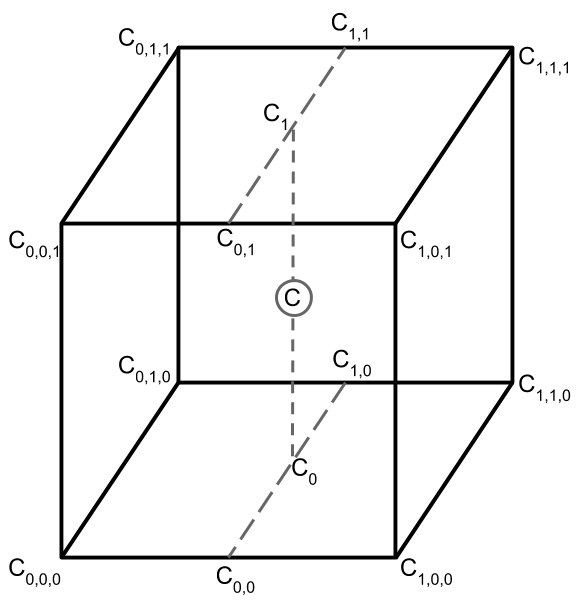
\includegraphics[width=0.6\textwidth]{images/trilinear_interpolation}
	\caption{Illustration of trilinear interpolation. The value at the point
	$C$ is linearly interpolated from the 8 corner points of the cube.}
	\label{fig:trilinearinterpolation}
\end{figure}

The boundary conditions for the wind velocity is described in \ref{chap:windsim}
in the Boundary Conditions section, the advected velocities are modified based on
the obstacles data and on the border of the volume the velocities are set to
predetermined values.

\subsection{Solve Poisson Equation}

The Poisson equation is solved using the KSP object from PETSc. KSP stands for
Krylov subspace methods, discussed in the background chapter.

\subsubsection{Creating the Linear System}

The linear system $Ax = b$ consists of the matrix $A$, and the vectors $x$ and
$b$. The vector $x$ is set to store the initial guess for the linear solver,
which was chosen to be null vector, $x = 0$. The vector $b$ is the divergence of
the result of the advected velocity field from the advection step, $b = \nabla
\cdot u^*$. How to calculate the values for $b$ is shown in chapter 
\ref{chap:windsim}, in the section on the Poisson equation.

The matrix $A$ is a sparse banded symmetric matrix. Before inserting values into
the matrix, storage was allocated for the matrix using the PETSc function
$MatSeqAIJSetPreallocation$. This increases the performance of the matrix
initialization by several orders of magnitude and is essential for large problem
sizes. If the storage is not preallocated, the matrix will be reallocated every
time a new value is inserted. For inserting values into the matrix, the function
$MatSetValuesStencil$ was used. This function was used to insert one row of 
values at a time. The values inserted are the coefficients of the pressure terms
derived in chapter \ref{chap:windsim}, in the section on the Poisson equation.

\subsubsection{Solver Setup}

\subsection{Projection}

During this step the advected velocity field is modified using the gradient of
the pressure field to calculate the final velocity field for the wind simulation.
The method used for this calculation is shown in chapter \ref{chap:windsim}.
